\chapterimage{back2.jpg} % Chapter heading image
\chapter{Introduction}

Developing safety critical applications often requires rare human resources to complete successfully, while off-the-shelf block solutions appear difficult to adapt especially during short-term projects. The CLEARSY Safety Platform fulfils a need for a technical solution to overcome the difficulties of developing SIL3/SIL4 system with its technology based on a double-processor and a formal method with proof to ensure safety at the highest level\cite{lecomte2016double}. The formal method, namely the B method\cite{Abrial.1996}, has been heavily used in the railway industry for decades\cite{DBLP:conf/fmics/Lecomte09}\cite{DBLP:conf/fm/Lecomte08}\cite{DBLP:journals/entcs/Benveniste11}. Using its IDE, Atelier B, to program the CLEARSY Safety Platform ensures a higher level of confidence in the generated software.\\

\begin{figure}[h]
\centering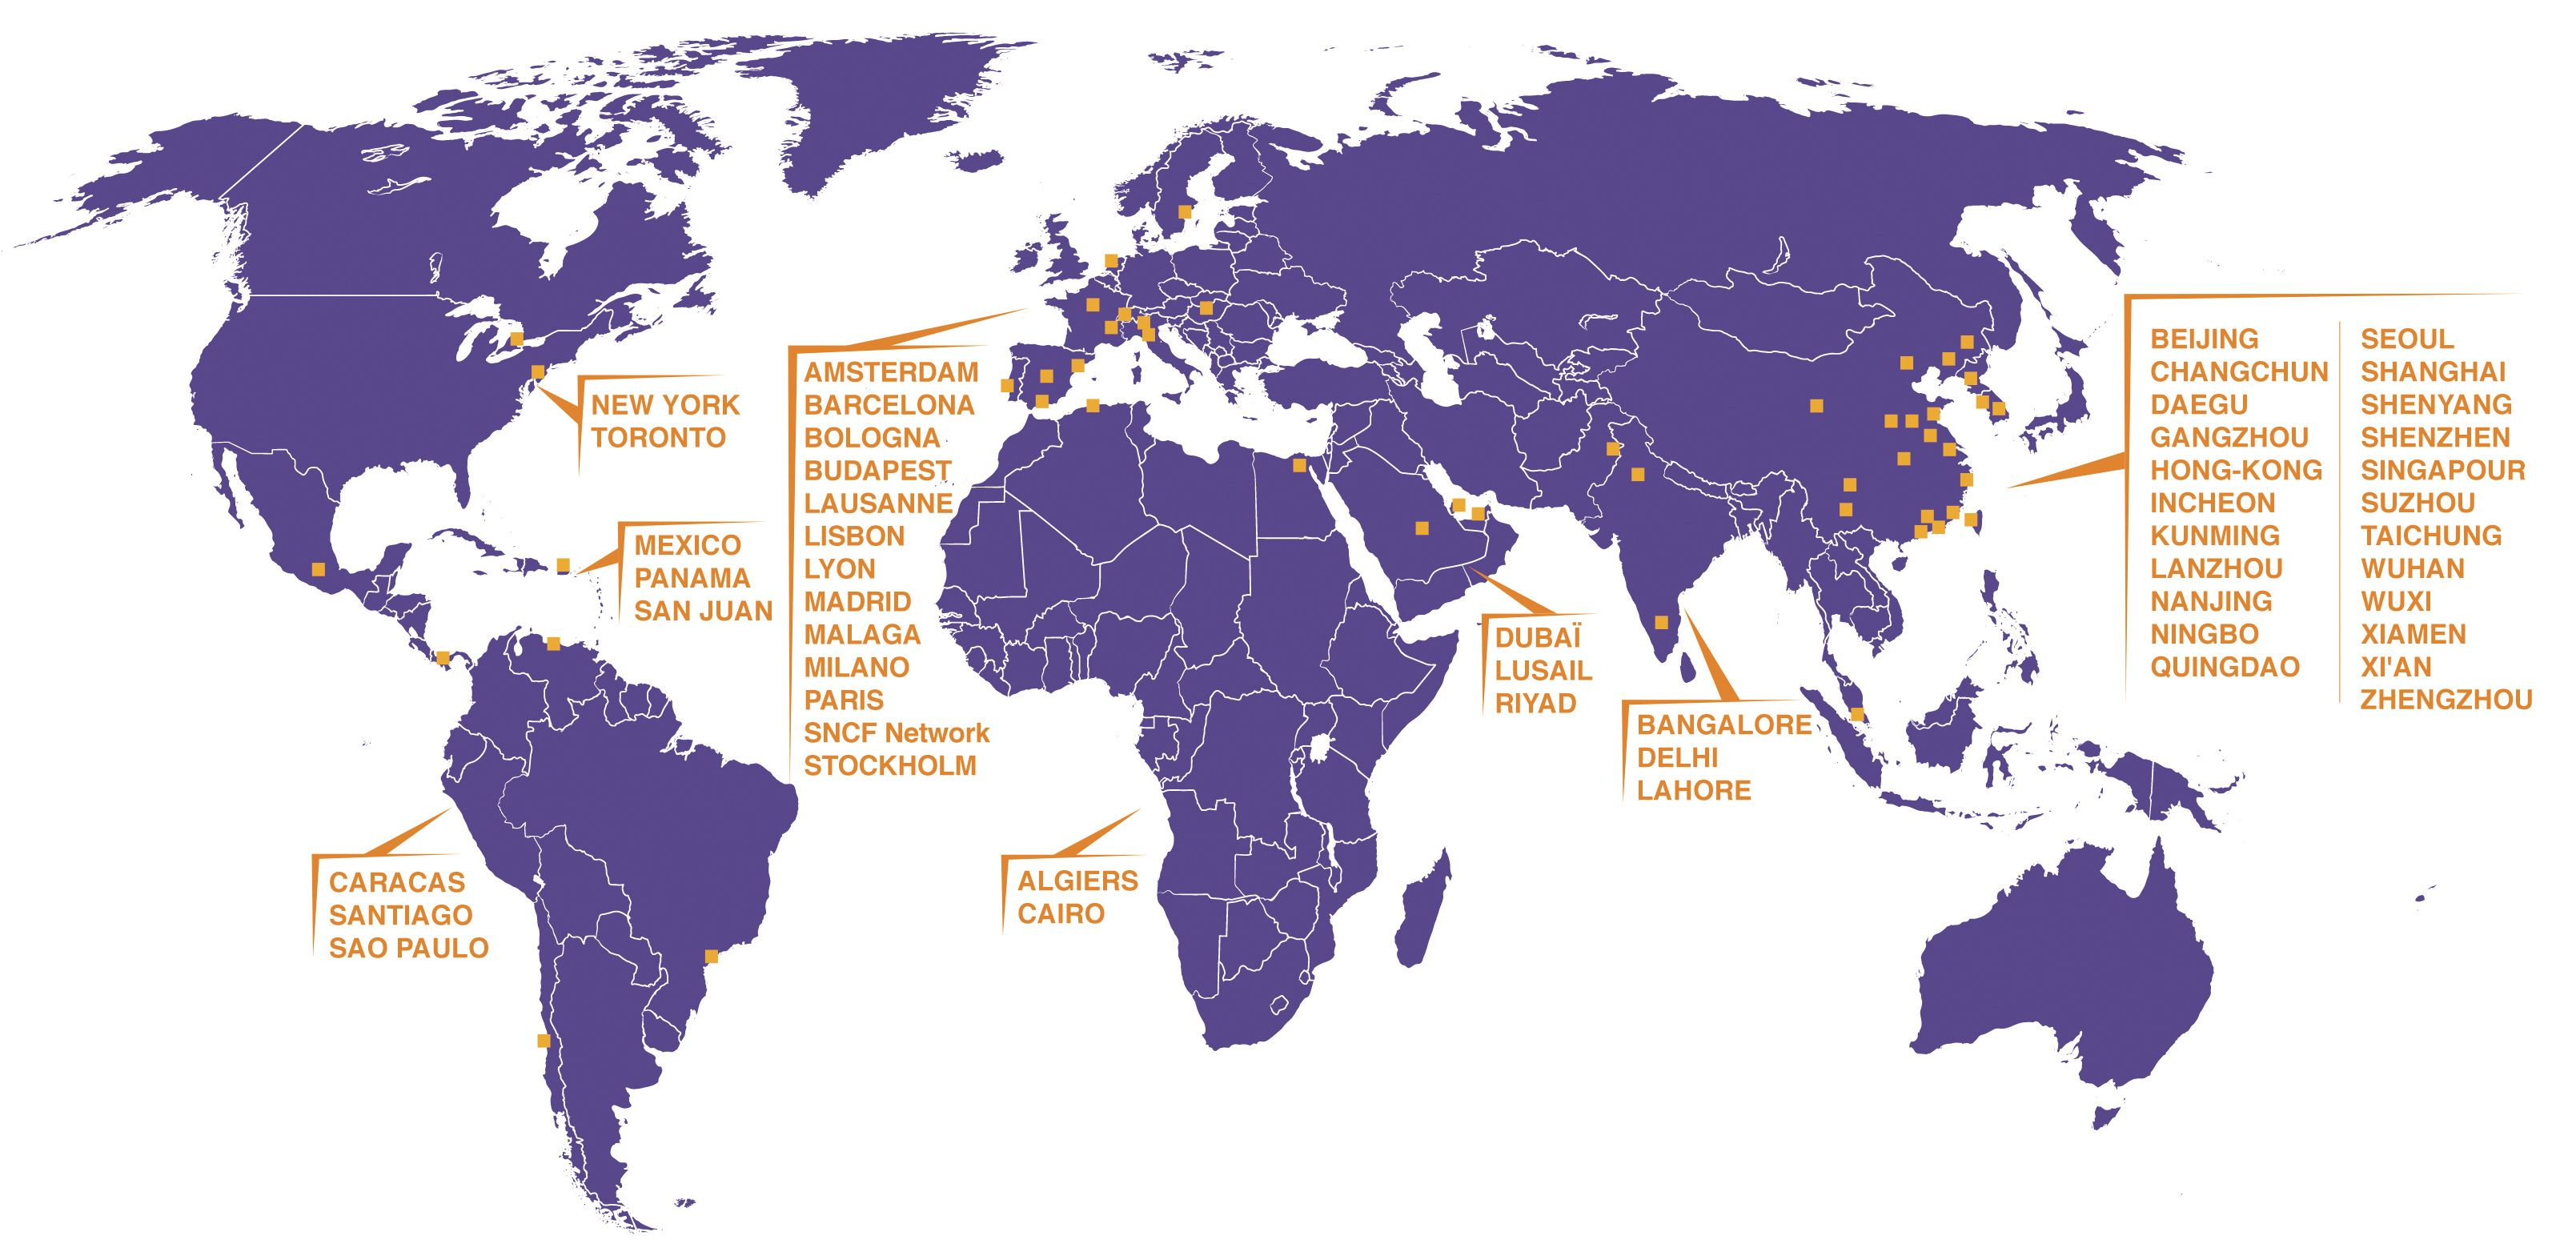
\includegraphics[scale=0.5]{Pictures/INTRO-AtelierB.jpg}
\caption{Metros and trains equipped with B SIL4 software}
\end{figure}

The CLEARSY Safety Platform is both a software and a hardware platform aimed at designing and executing safety critical applications. One formal modelling language is used to program the board. Programs are developed using the dedicated IDE or could be the by-product of some translation from a Domain Specific Language to B. The IDE takes care of the verification of the software (type check, proof, compilation) and then ensures its upload to the hardware platform. The program is guaranteed to execute until a misbehaviour is detected, leading to a safe restricted mode where board outputs are deactivated.\\

The CLEARSY Safety Platform eases the development of safety critical applications as:
\begin{itemize}
    \item it covers the whole development cycle,
    \item the safety principles are built-in and are out of reach of the developer, who cannot alter them,
    \item it is based on a formal language (B) and related proof tools,
    \item the mathematical proof replaces unit and integration testing.\\
\end{itemize}

%
The CLEARSY Safety Platform eases the certification of safety critical applications as:
\begin{itemize}
    \item the safety cannot be altered by the developer,
    \item it will come with a certification kit.\\
\end{itemize}

The building blocks of the CLEARSY Safety Platform, already certified in international projects during the years 2017 and 2018 by several certification bodies, have been used to develop a generic version of this technology that could fit a broader range of applications. 

\begin{figure}[h]
\centering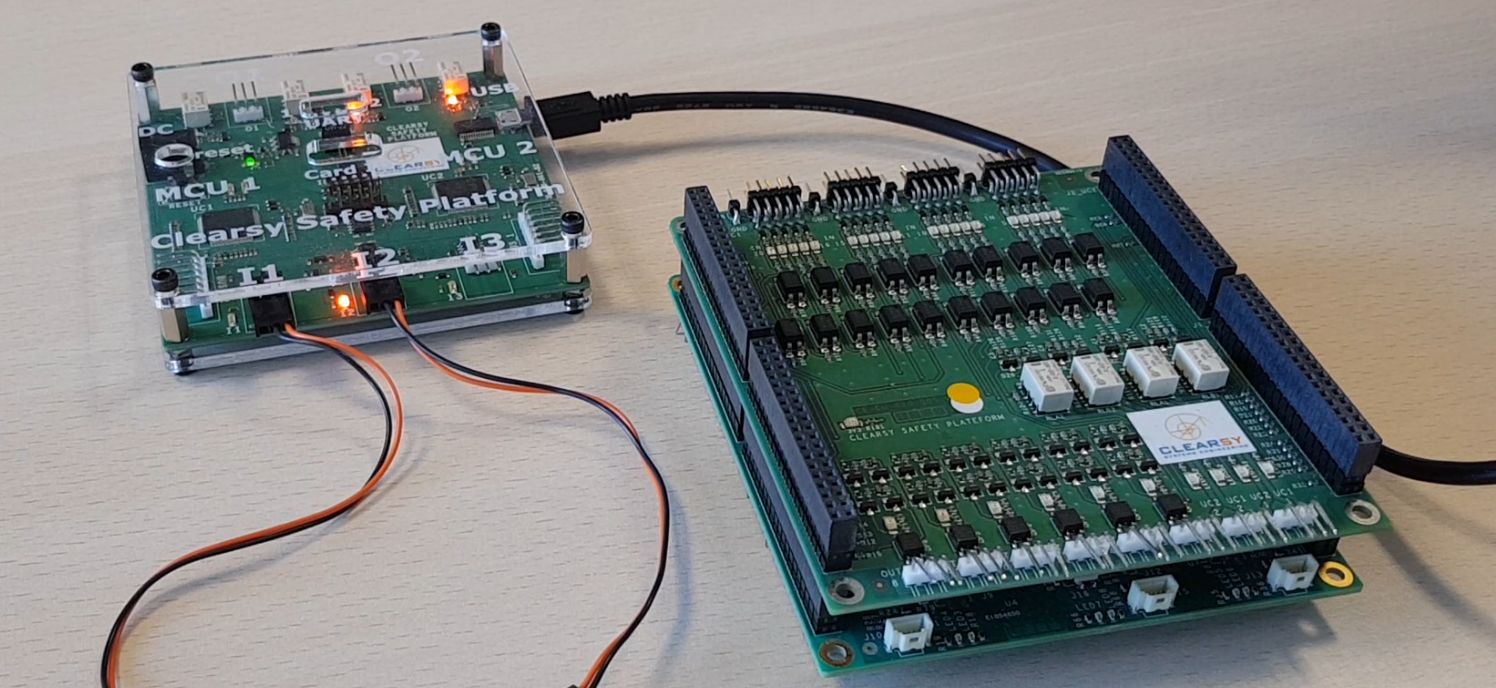
\includegraphics[scale=0.25]{Pictures/INTRO-SK0+SK1.jpg}
\caption{Starter kits SK$_0$ (left) and SK$_1$ (right)}
\end{figure}

The first starter kit, SK$_0$, allows to experiment with the whole development chain, including the IDE, using the B-Method and an electronic board hosting the safe execution platform relying on two PIC32 microcontrollers, providing 3 digital inputs and 2 digital outputs.\\

The second starter kit, SK$_1$, is functionally identical to SK$_0$. It provides 20 digital inputs and 8 digital outputs. The core automaton, with its two PIC32 microcontrollers, is hosted on a motherboard while the inputs/outputs are located on a daughterboard.

